\documentclass{article}
\usepackage{amsfonts,amssymb}
\usepackage[margin=1in]{geometry}
\usepackage{tikz}
\usepackage{graphicx}
\usetikzlibrary{arrows,automata,positioning}

\title{CSCI 480, Winter 2016\\Math Exercises \# 4}
\author{Andrew Nguyen}
\date{Due date:  }

\begin{document}

\maketitle

\begin{itemize}
  \item
Build deterministic finite automata and/or regular expressions (as
requested) for each of the languages in questions \ref{langfirst} to
\ref{langlast}.  Create simple, meaningful automata and regular
expressions (rather than, {\em e.g.}, using the algorithm to create a
regular expression from a DFA) and explain how they work.  In all
cases the alphabet is $\Sigma = \{0,1\}$.
\item
DFAs should be specified with pictures, preferably
typeset with {\bf TikZ}, not tables
(as tables are very hard to read).  Try to typeset them so that the
labels on the arcs are clear, {\em etc.}
\item
If you are having a difficult time with {\bf TikZ}, clear, legible
hand-drawn figures (or figures created with a drawing program)
are acceptable as graphics inclusions into your \LaTeX\ 
documents. 
\end{itemize}


For solutions to problems 1 – 6, see figures 1, 2, and 3 at the very bottom.

\begin{enumerate}
\item
  \label{langfirst}
  The language $\{100, 10, 011\}$.
  Regular expression: 
  
  

\item   The language $\{100, 10, 011\}$.
  DFA:
  

\item The set of 
  all strings that begin or end with a doubled digit, either 11 or 00.
  Regular expression:

  
\item The set of 
  all strings that begin or end with a doubled digit, either 11 or 00.
  DFA:
  
  
\item
The set of all strings that have exactly one doubled digit in them.
  In other words, either 11 or 00 occurs in the string, but not both,
  and it only occurs once.
  Regular expression:
  

\item \label{langlast}
The set of all strings that have exactly one doubled digit in them.
  In other words, either 11 or 00 occurs in the string, but not both,
  and it only occurs once.
DFA:

\item Use the pumping lemma to show that the language that consists of
  all {\em palindromes} over $\Sigma=\{0,1\}$ is not regular.  A palindrome
  is a string that reads the same backwards and forwards, for example
  11011, 01010, 0, and 0110.
  \[ L = \{w \in \{0,1\}^* \mid w = w^R\}\]
  
  1) Suppose that L is regular. L then, must satisfy the pumping lemma.
  
  2) $\exists p$, the pumping length, such that:
  
  3) $\exists S \in L$, $|S| \geq p$
  
  4) $S = xyz$, $y \neq \epsilon$
  
  5) $\exists i \geq 0$ $|$ $xy^iz \notin L$
  
  6) $|xy| < p$
  
  Suppose $S = 0^p1^p0^p$, since $|xy| < p$, we know that the substring $xy$ must fall into the first $p$
  symbols of the string. 
  
  This means that for the string $S$, $xy$ will consist of only 0's, with $z$ being the rest of the string.
  
  If $i = 0$, then $xy^0z = xz$. 
  
  $xz = 0^{p-|y|}1^p0^p$
  
  After $y$ is pumped to $i = 0$ times, the string no longer has an even number of 0's on both sides of the 1's in the middle.
  String S fails to satisfy the palindrome requirement of the language, and thus is not in the language. 
  
  By contradiction then, L is not a regular language.
  
  

\item Use the pumping lemma to show that the following language is not
  regular.  For examples, 00110000, 01110000 and 00 are in the
  language, but 110 is not.
  \[ L = \{0^i1^j0^{i+j} \mid i,j\in\{0,1,2,\ldots\}\} \]
  
  1) Suppose that L is regular. L then, must satisfy the pumping lemma.
  
  2) $\exists p$, the pumping length, such that:
  
  3) $\exists S \in L$, $|S| \geq p$
  
  4) $S = xyz$, $y \neq \epsilon$
  
  5) $\exists i \geq 0$ $|$ $xy^iz \notin L$
  
  6) $|xy| < p$
  
  Suppose $S = 0^p1^{p+1}0^{2p+1}$. Since $|xy| < p$, then the substring $xy$ must fall into the first p symbols of the input string. In this case, $xy$ would be comprised of only 0's from the first $0^p$ zeroes. $z$ comprises the rest of the string.
  
  Suppose that we pump $y, i = 0$ times. $xy^0z = xz$,
  
  $xz = 0^{p-|y|}1^{p+1}0^{2p+1}$
  
  By contradiction, the language L is not regular because the string $xz$ does not follow the rule $0^i1^j0^{i+j}$ and 
  is not in the language as a result.
  


\item Give an example of a regular language $R$ and a nonregular
  language $N$ such that $R\cup N$ is regular.  Describe all three
  languages in English and either prove they are regular/nonregular,
  or show that they are instances of languages with known regularity.
  
  The collection of regular languages over an alphabet Σ is defined recursively as follows:

	1) The empty language $\emptyset$ is a regular language.
	2) For each a ∈ Σ (a belongs to Σ), the singleton language {a} is a regular language.
	3) If A and B are regular languages, then A ∪ B (union), A • B (concatenation), and A* (Kleene star) are regular languages.
	4) No other languages over Σ are regular.
	-Wikipedia page on regular languages
  
  All finite languages are regular. This means that the smallest regular languages are:
  $\emptyset, \{\epsilon\}, \{0\}, \{1\}, etc.$
  Note that $\sum^*, (where \sum = \{0,1\}), \{0\}, \{1\}, etc.$ is also a regular language.
  Any language that can be represented via a regular expression is also regular.
  
  Suppose there is a language $L_1 = \{w \in \sum | w = 0^n1^n, n \geq 0\}$, which is non-regular (because it has an infinite and uncountable number of substrings for all $n$).
  
  Additionally, there is a language $L_2 = \{0^n1^m | n, m \geq 0\}$. $L_2$ is regular because $n$ and $m$ do not have to be equal,
  and thus can satisfy the pumping lemma. 
  
  $L_1 \cup L_2 = L_2$. The reason for this is that $L_1$ is merely a subset of $L_2$ where the variables $m$ and $n$ happen to
  be equal. The resulting language is regular.
  
  Proof for $L_1 = \{w \in \sum | w = 0^n1^n, n \geq 0\}$:
  
  	By pumping lemma:
  	
  		Suppose $L_1$ is regular, $S \in L_1$ and $|S| \geq p$.
  		$S = xyz, i \geq 0 $ and $y \neq \epsilon$.
  		$S = xyz = 0^p1^p$, since the P.L. states that $|xy| < p$, then $xy$ must fall into the first $p$ symbols of the string,
  		making $xy$ comprised of only 0's in this string. 
  		
  		If we pump $y^i, i = 0$ times, then the string $xy^0z = xz = 0^{p-|y|}1^p$
  		
  		Then $xz$ no longer satisfies the rule of the language $0^n1^n$, and is therefore not in the language. 
  		
  		By contradiction, $L_1$ cannot be a regular language.
  		
  		
  Proof for $L_2 = \{0^n1^m | n, m \geq 0\}$:
  	
  	By pumping lemma:
  	
  		Suppose $L_2$ is regular, $S \in L_2$ and $|S| \geq p$.
  		$S = xyz, i \geq 0 $ and $y \neq \epsilon$.
  		$S = xyz = 0^p1^p$, since the P.L. states that $|xy| < p$, then $xy$ must fall into the first $p$ symbols of the string,
  		making $xy$ comprised of only 0's in this string. 
  		
  		If we pump $y^i, i = 0$ times, then the string $xy^0z = xz = 0^{p-|y|}1^p$
  		
  		The substring $xz$ still satisfies the rule of the language $0^n1^m$, so long as both $n$ and $m$ are greater than zero,
  		and therefore is still in the language. Merely satisfying the pumping lemma does not make a language regular though.
  		
  		However, because $L_2$ can be represented by the regular expression $0^*1^*$, it is in fact a regular language.
  		

\item Give an example of a regular language $R$ and a nonregular
  language $N$ such that $R\cup N$ is nonregular. Describe all three
  languages in English and either prove they are regular/nonregular,
  or show that they are instances of languages with known regularity.

  All finite languages are regular. This means that the smallest regular languages are:
  $\emptyset, \{\epsilon\}, \{0\}, \{1\}, etc.$
  Note that $\sum^*, (where \sum = \{0,1\}), \{0\}, \{1\}, etc.$ is also a regular language.
  Any language that can be represented via a regular expression is also regular.

  
  Suppose there is a language $L_1 = \{w \in \sum | w = 0^n1^n, n \geq 0\}$, which is non-regular (because it has an infinite and uncountable number of substrings for all $n$). This is the same language used in 9), the proof is there.
  
  There is another language, $L_2 = \{0, 1\}$ that is regular (because it is finite and countable).
  
  $L_1 \cup L_2 = \{0, 1\}L_1$ The resulting language is non-regular, because even with the concatenation of $\{0,1\}$, the $L_1$
  portion is still non-regular by definition, making the language resulting from the union also non-regular. 
  
  Another example would be to simply replace $L_2$ with the empty set. 
  
  $L_1 \cup \emptyset = L_1$, which still remains non-regular.
  
  
  \begin{figure*}[b!]
  
  	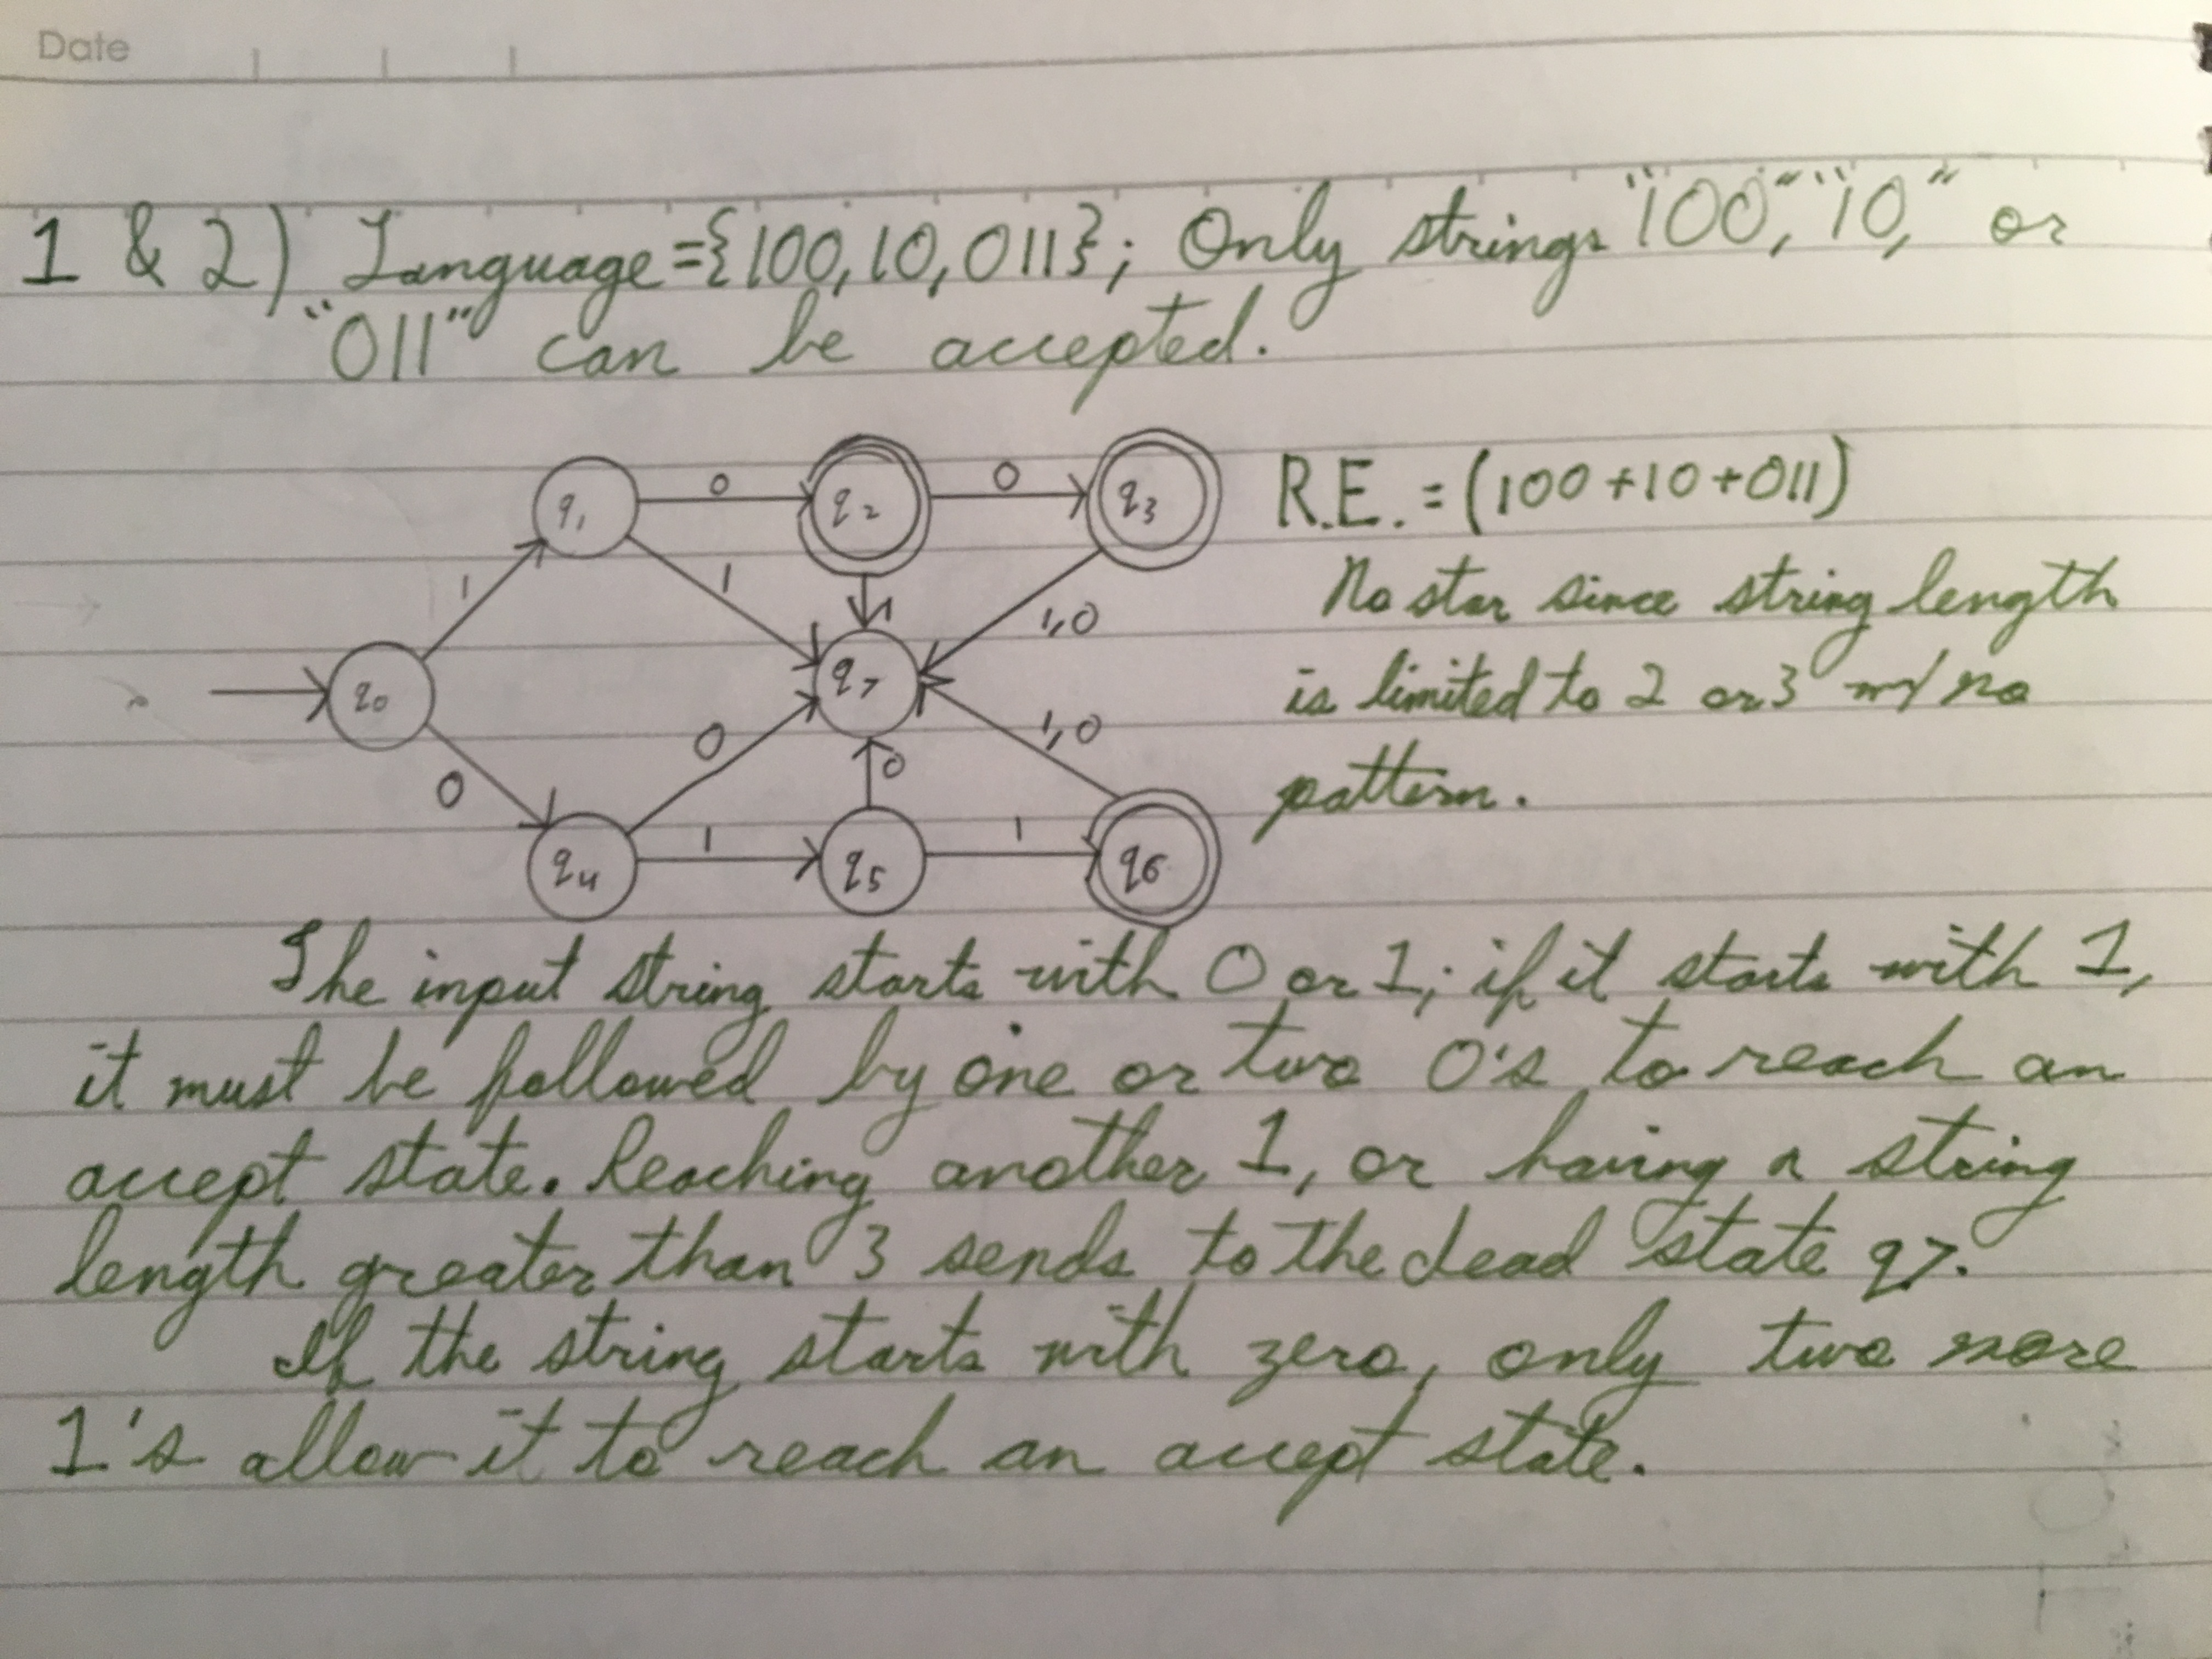
\includegraphics[width=\linewidth]{Math041&2}
  	\caption{Figure 1 for questions 1 \& 2}

  \end{figure*}
  
  \begin{figure*}[b!]
  
  	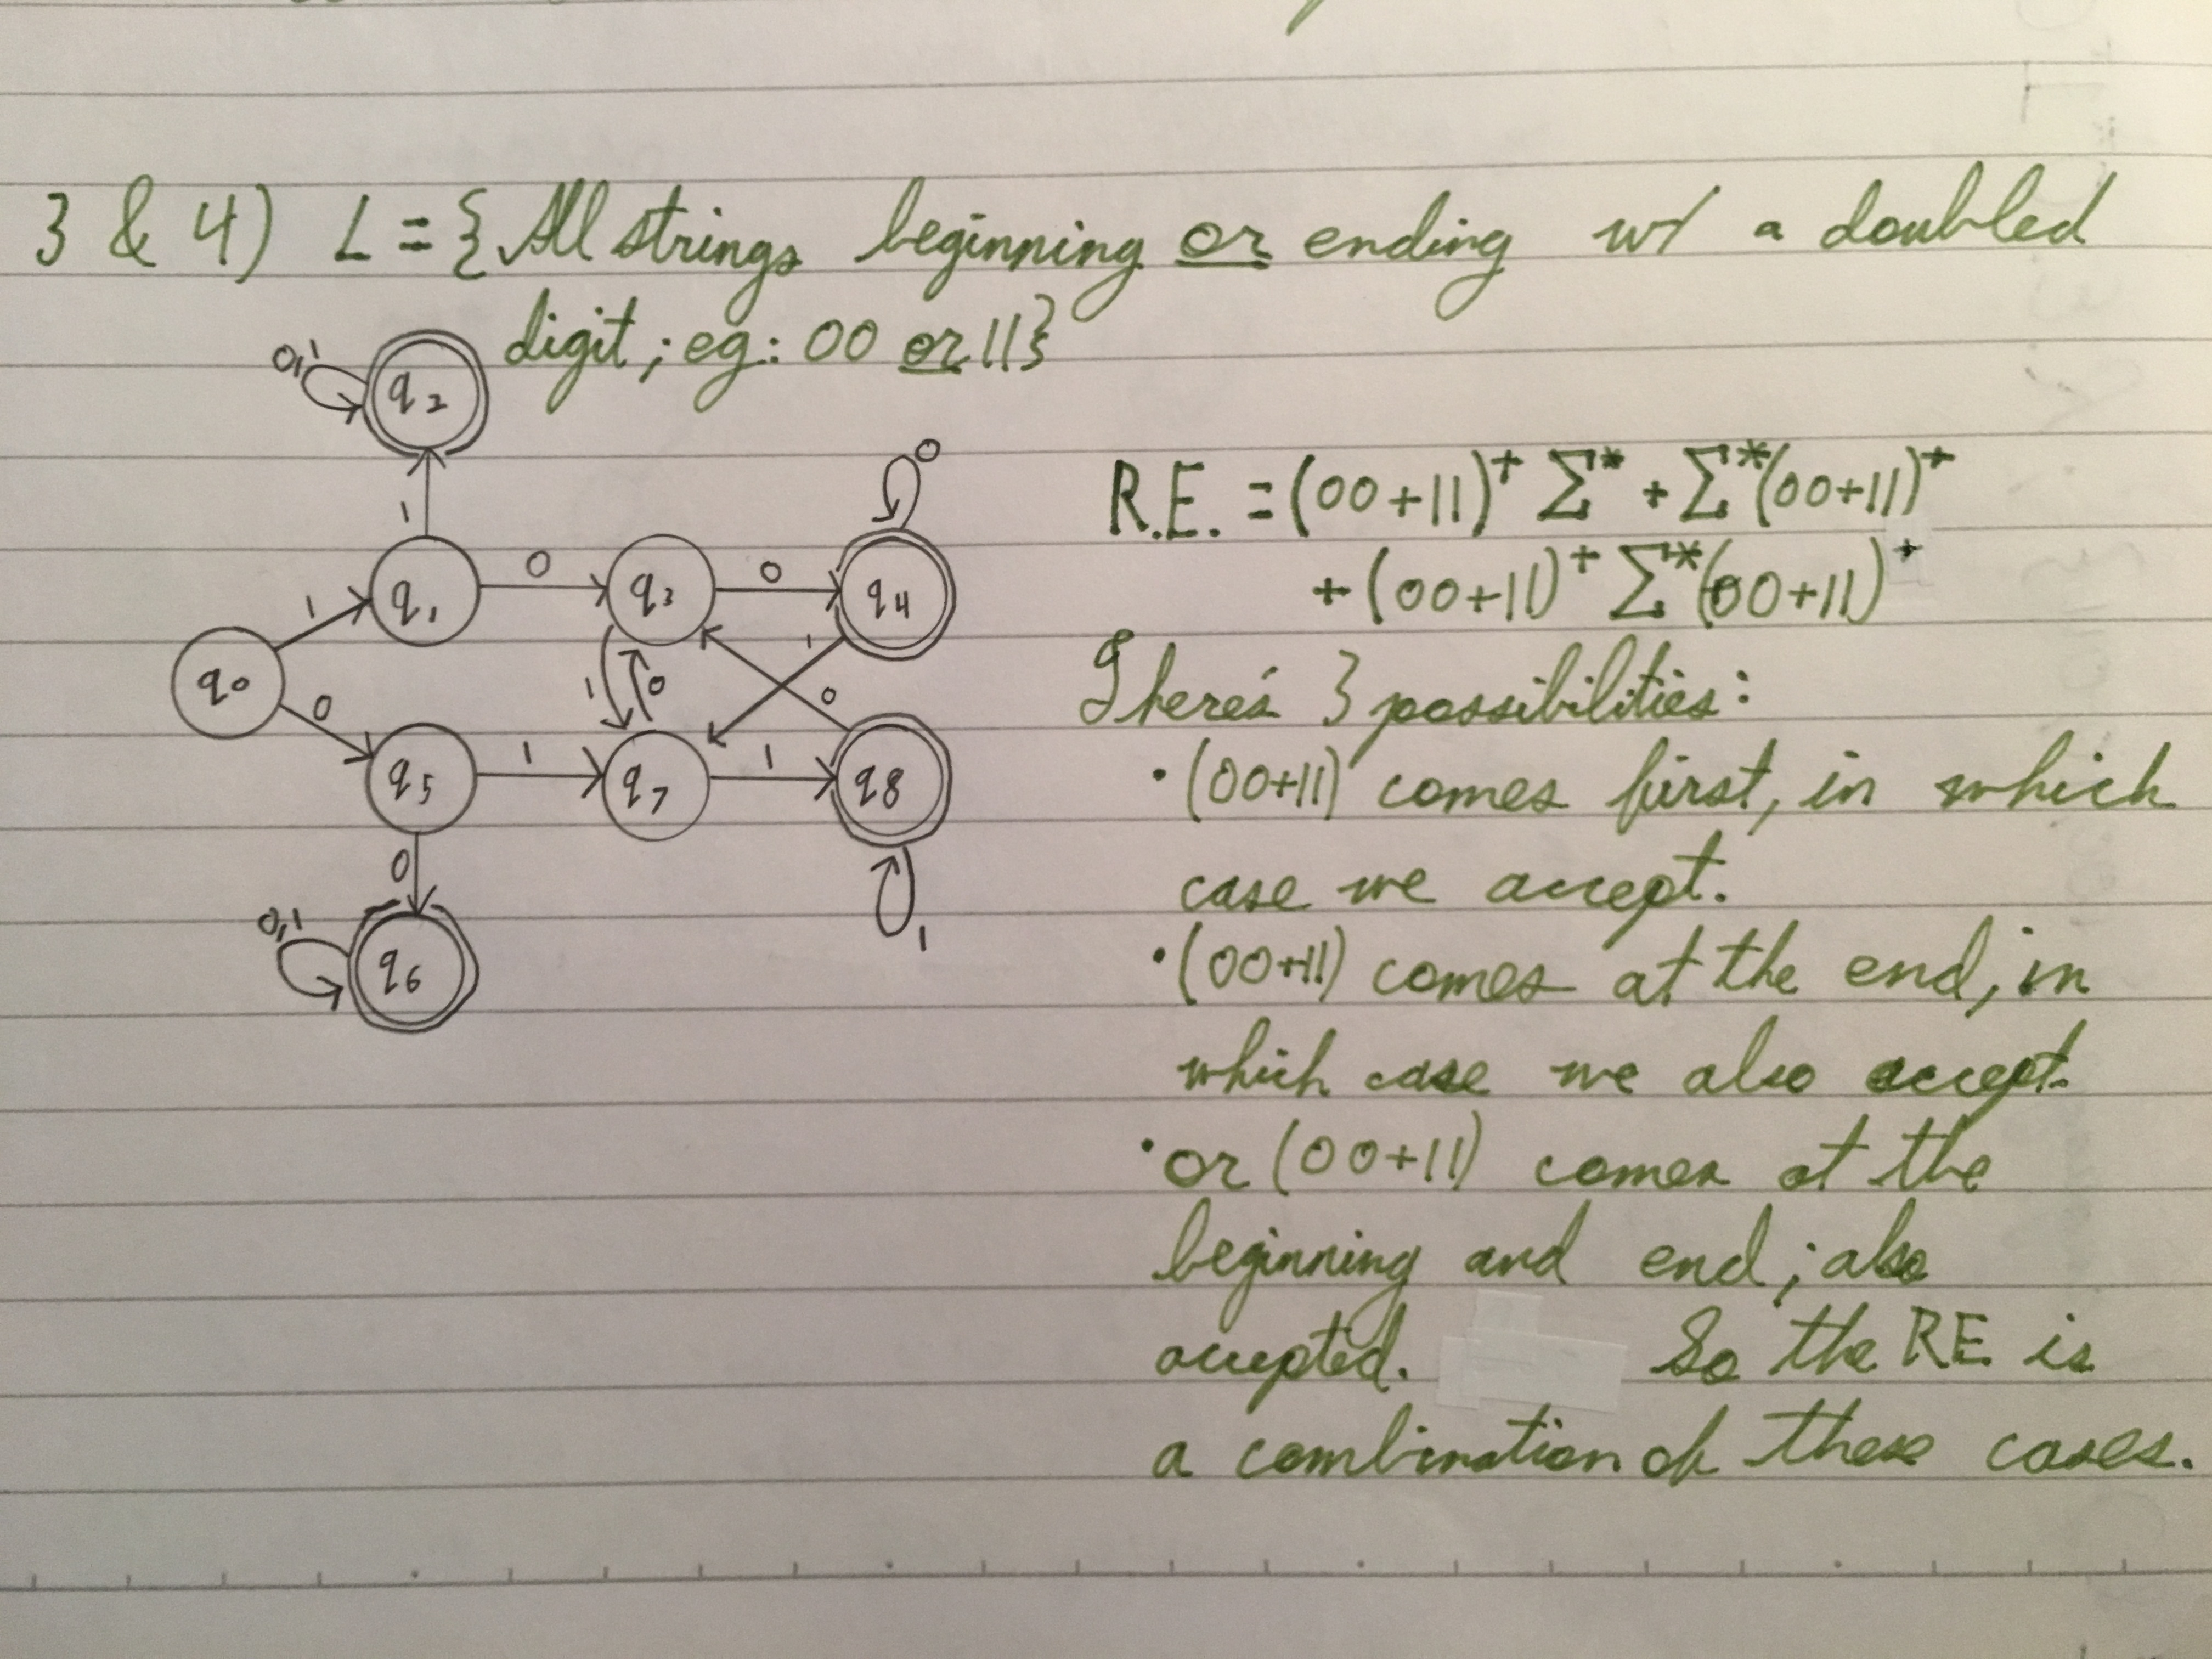
\includegraphics[width=\linewidth]{Math043&4}
  	\caption{Figure 2 for questions 3 \& 4}

  \end{figure*}
  
  \begin{figure*}[b!]
  
  	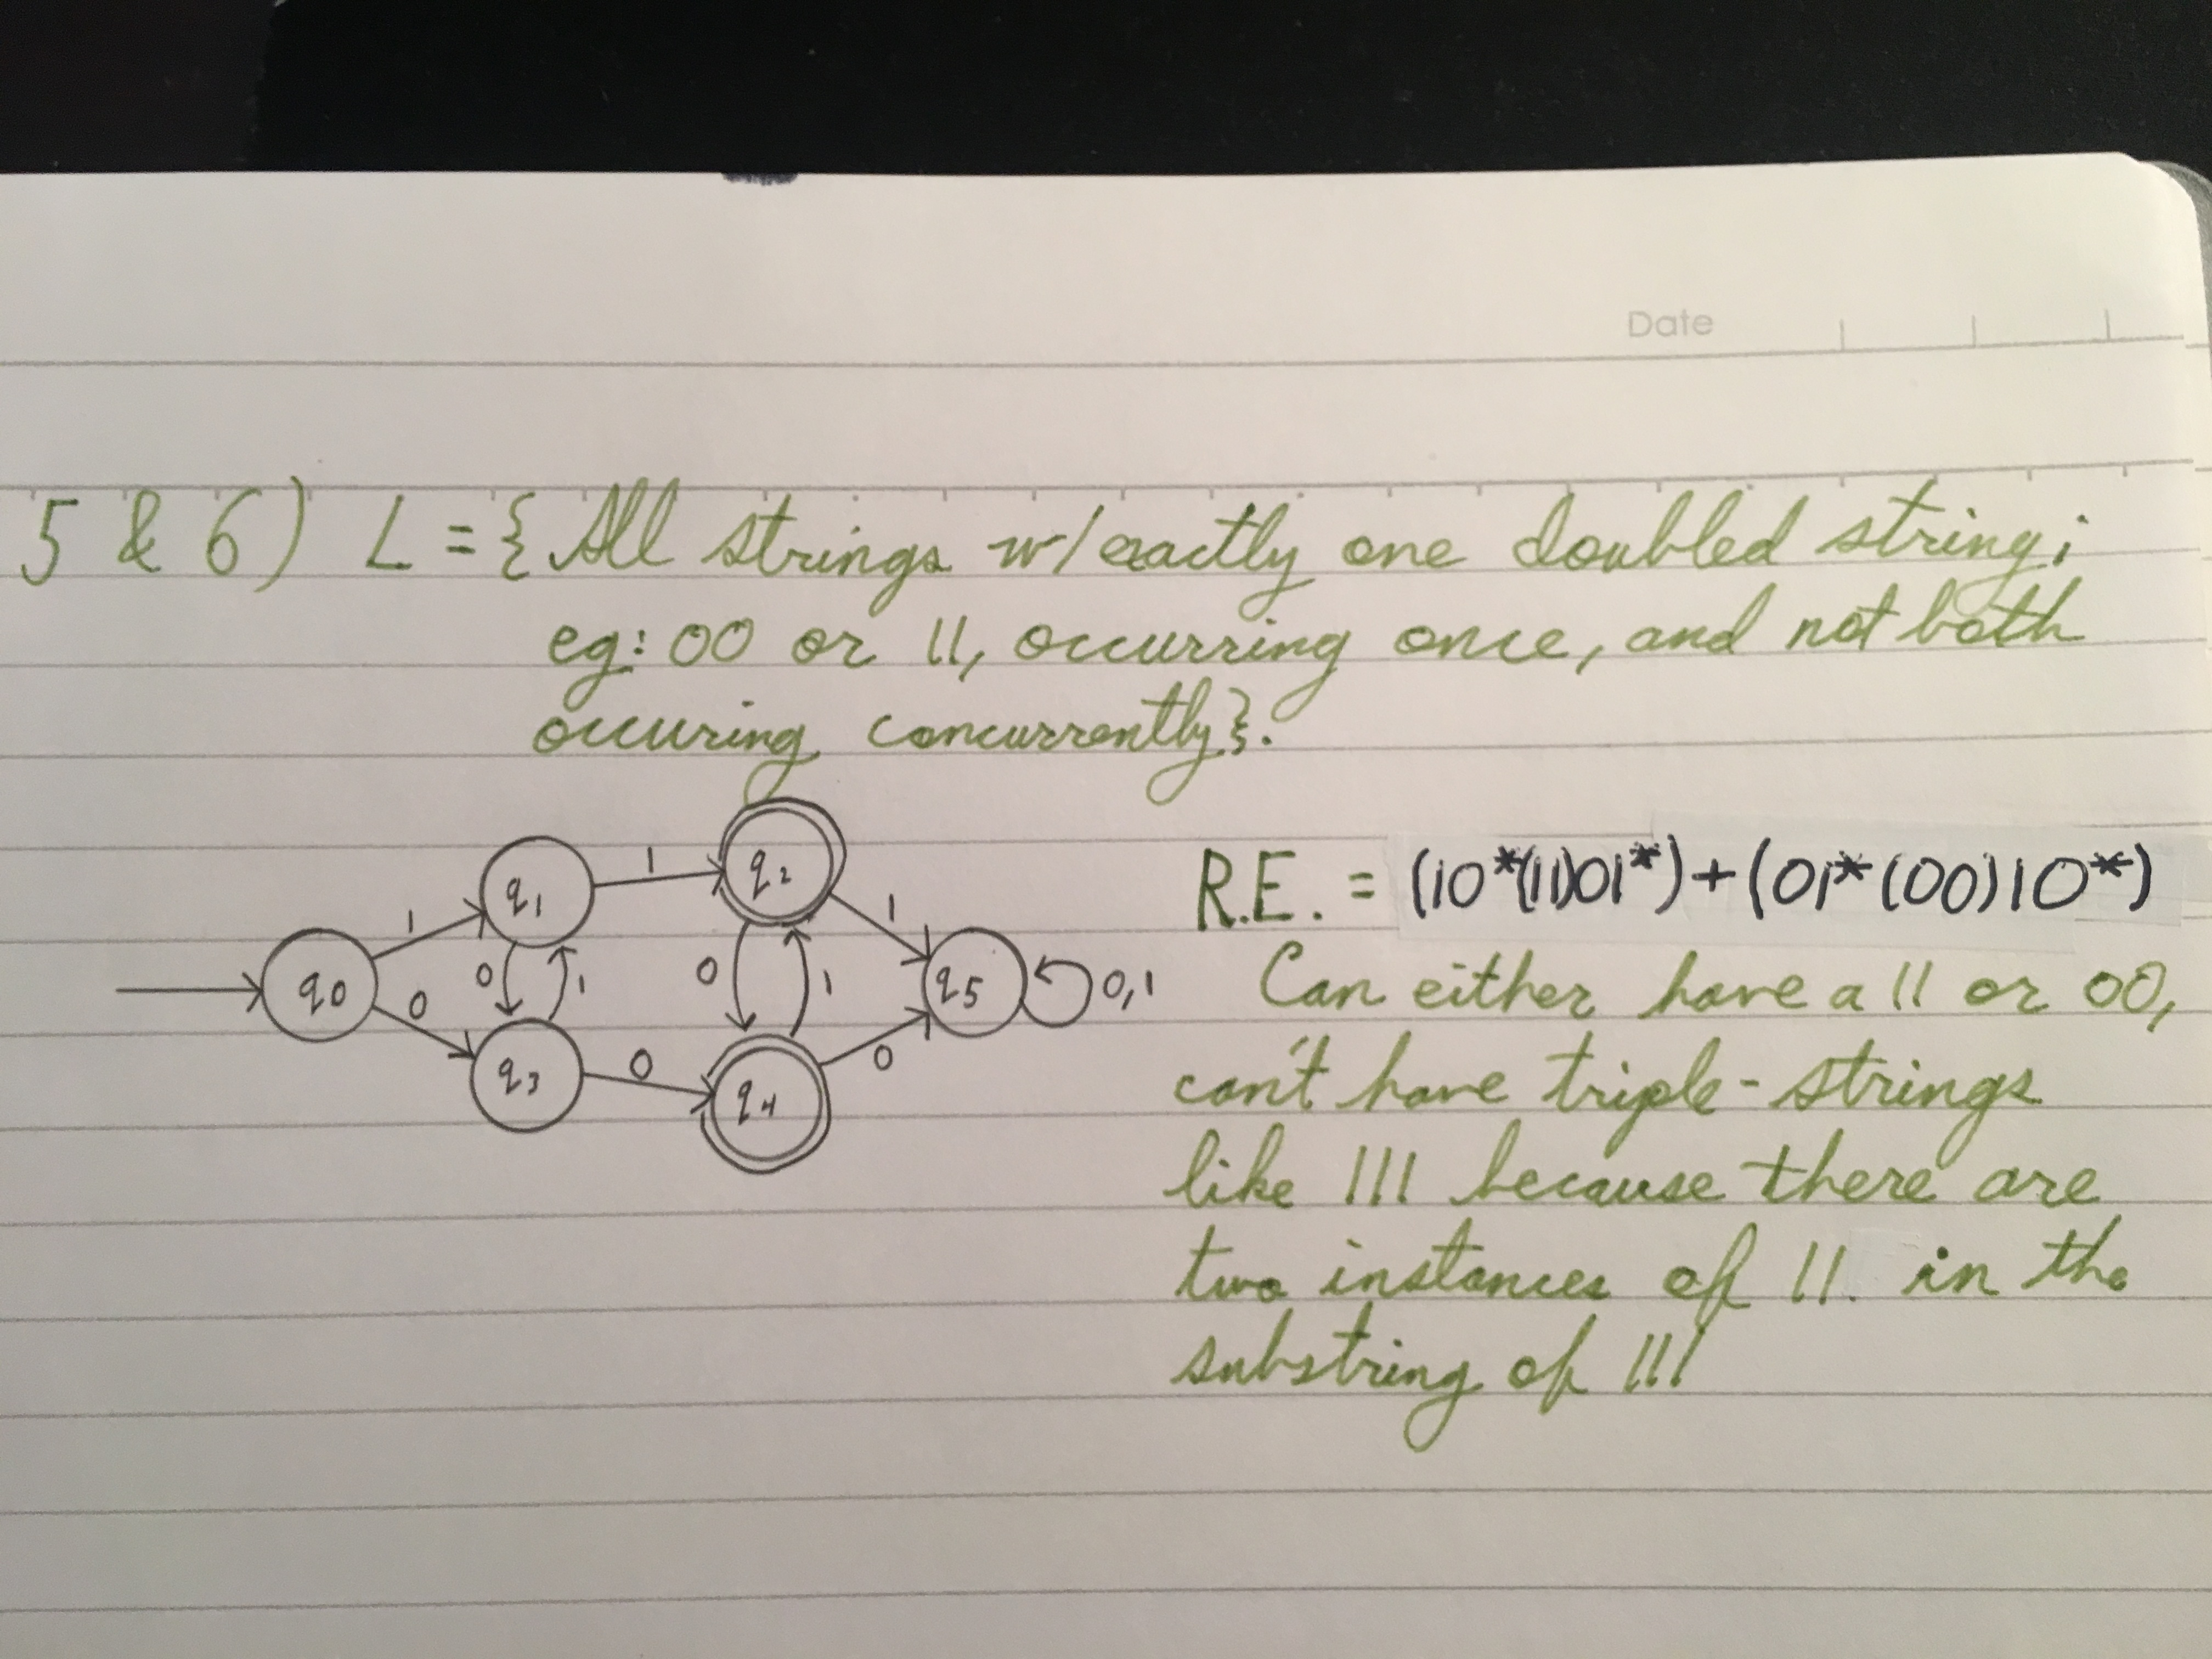
\includegraphics[width=\linewidth]{Math045&6}
  	\caption{Figure 3 for questions 5 \& 6}

  \end{figure*}


\end{enumerate}


\end{document}